\section{Geographical and stratigraphic distribution of body size data}

Body size data was available from all four continents, were testudinidae occur, and over a time period of 20 mya (Fig. \ref{fig:mapBS}, Table \ref{tab:bins}).

--> samples all over the world and over the whole time period with more or less equally distributed sample sizes (over time bins, continents are uneven --> see SAC)





%______________________________________________________________________
\begin{figure}[htbp]
	\centering
	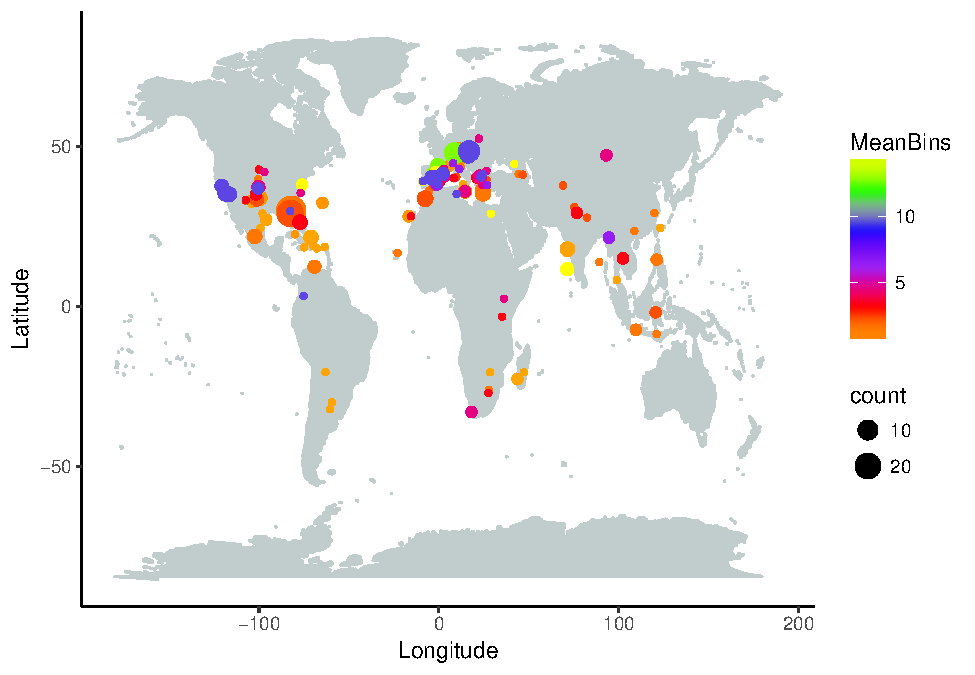
\includegraphics[width=\textwidth]{MA_JJ_files/figure-latex/MapCL-1.pdf}
	\caption[Map: body size localities]{Map displaying all localities for which body size data for testudinids was available in the literature. Size of points denotes sample size, color denotes approximate age.}
	\label{fig:mapBS}
\end{figure}
